\documentclass[a4paper,10pt]{article}
\usepackage{graphicx}
\usepackage{amsmath}
\usepackage{amssymb}
\usepackage[italian]{babel}
\usepackage[T1]{fontenc}
\usepackage[utf8]{inputenc}
\usepackage[margin=1.25in]{geometry}
\usepackage{caption}
\usepackage{subcaption}

\usepackage[backend=biber]{biblatex}
\addbibresource{ref.bib}

\begin{document}

   \title{{\large Università degli Studi di Padova \\ } {\normalsize Corso di laurea triennale in Ingegneria Informatica}\\ \vspace{1.8cm} \textbf{ Homework 2}\\{\normalsize Strumenti per la valutazione delle prestazioni di rete}}

   \maketitle
   \vspace{7.2cm}
   \renewcommand{\contentsname}{Indice}      
   \tableofcontents
   \newpage

\section{Comando \texttt{ping} }
\texttt{ping} (Packet INternet Groper) è un software di amministrazione per reti di computer utilizzato per verificare la raggiungibilità di un host all'interno di una rete IP. Questa applicazione è supportata nella maggior parte dei sistemi operativi comuni ed è ampiamente utilizzata come strumento elementare di diagnostica di rete. \\\\
Il funzionamento di \texttt{ping} è interamente basato sul protocollo ICMP (Internet Control Message Protocol, RFC 792), che si appoggia direttamente ai servizi offerti dall'Internet Protocol, senza coinvolgere alcun tipo di servizio di livello di trasporto. L'applicazione invia una serie di pacchetti ICMP Echo Request ad una destinazione, la quale risponde ad ogni pacchetto ricevuto inviando un corrispettivo pacchetto ICMP Echo Reply di risposta della stessa dimensione della richiesta. Una rappresentazione grafica della struttura di un pacchetto ICMP è riportata in Figura \ref{fig:ICMP}. \texttt{ping} misura il cosiddetto \textit{Round-Trip Time} (RTT), ovvero il tempo che intercorre tra l'invio della richiesta e la ricezione della risposta, per poi visualizzarlo in output.

\begin{figure}[h!]
	\centering
	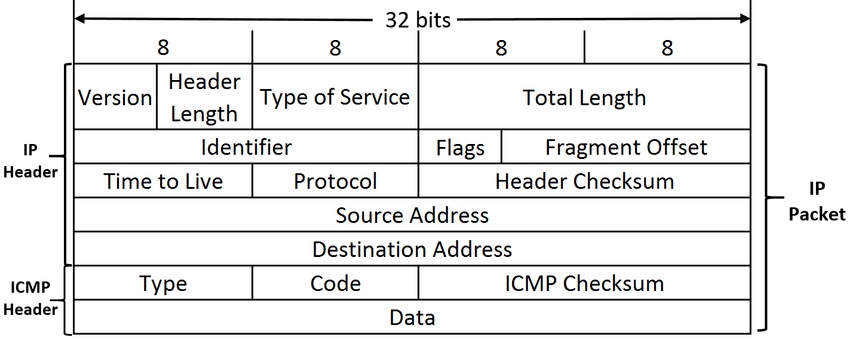
\includegraphics[scale=0.25]{img/icmp.png}
  	\caption{Struttura pacchetto ICMP \cite{ref:icmp}}
  	\label{fig:ICMP}
\end{figure}

\subsection{Opzioni da linea di comando}
Il software \texttt{ping} offre numerose opzioni da linea di comando, che possono variare a seconda del sistema operativo in cui è implementato e dei privilegi posseduti dall'utente che lo invoca. Una lista delle opzioni disponibili può essere ottenuta dall'utente mediante l'invocazione del comando \texttt{man ping}. Per quanto riguarda le opzioni che permettono l'attivazione di specifiche funzionalità definite nella consegna, ne è stata verificata l'esistenza e riportato il formato di seguito.
\begin{itemize}

\item \textbf{\texttt{-c count}}: dopo aver inviato \textit{count} pacchetti ECHO REQUEST, ne interrompe l'invio, rimanendo in attesa dei \textit{count} pacchetti ECHO REPLY (se utilizzato insieme ad opzioni che permettono di specificare una deadline, \texttt{ping} aspetta al massimo fino a che il timeout non termina e alcune request potrebbero non ricevere risposta) 

\item \textbf{\texttt{-s packetsize}}: specifica il numero di data byte da inviare. Il default corrisponde a 56 data bytes, che si traducono in una dimensione totale del pacchetto di 64 ICMP data bytes considerando anche gli 8 bytes dell'header. Si ricorda inoltre che la dimensione dei pacchetti IP è in ogni caso maggiore rispetto a questa, in quanto vengono aggiunti 20 bytes di header IP.

\item \textbf{\texttt{-t ttl}}: permette di definire il campo \textit{Time-To-Live} (TTL) dell'header IP. 

\end{itemize}

\newpage
\subsection{Time-To-Live}
Il \textit{Time-To-Live} (TTL) è una campo dell'header IP che viene impostato dal mittente e decrementato ogni volta che il pacchetto è inoltrato da un nodo intermedio nella rete. Se un nodo che non è il destinatario finale riceve un pacchetto il cui TTL è pari ad 1, il campo è decrementato ed il pacchetto scartato. Pertanto, il TTL determina il numero di inoltri (hop) che un pacchetto può subire prima di raggiungere la destinazione.\\\\
Al fine di testare il numero di hop che separano la macchina da cui sono stati svolti gli esperimenti dal server destinazione (88.80.187.84) è stato scritto un breve script di shell Linux, riportato di seguito.
\small
\begin{quote}
\begin{verbatim}
echo "Time-To-Live Experiment" > ttl.txt
for i in  8 9 10 11 12 13 14 15 
do
  echo "TTL $i" >> ttl.txt
  ping -q -c 15 -t $i 88.80.187.84 >> ttl.txt
done
\end{verbatim}
\end{quote}
\normalsize
Questo script permette di testare il comando \texttt{ping} specificando diversi valori di TTL $\in[8, 15]$ (mediante l'opzione \texttt{-t}) e di salvare i risultati ottenuti in un file denominato \texttt{ttl.txt}. Sono state inoltre utilizzate le opzioni \texttt{-q} per ridurre l'output del programma al minimo e \texttt{-c 15} per specificare il numero di pacchetti ICMP inviati per ogni esecuzione del programma. In questo modo è stato possibile verificare il valore di soglia per cui i pacchetti smettono di essere scartati da nodi intermedi e arrivano effettivamente al server destinazione. \\\\
Il valore di \textit{hop} tra la macchina mittente e il server di destinazione è stato quindi sperimentalmente verificato essere pari a \textbf{13}.

\newpage
\subsection{Round-Trip Time}
\label{par:x}
Il \textit{Round-Trip Time} (RTT) è definito come la somma dei ritardi accumulati nel percorso di andata (tra sorgente e destinazione) e di ritorno (viceversa) dai pacchetti ICMP. Numerando da 1 a \textit{n} i nodi attraversati durante l'intero tragitto comprensivo di andata e ritorno, il RTT del \textit{k}-esimo scambio request-reply può essere calcolato come
\begin{align}
RTT(k) = \sum_{i=1}^{n}  \left( \frac{L(k)}{R_i} + q_i(k) + \tau_i \right) + \sum_{j=1}^{m}  \left( \frac{L(k)}{R_j} + q_j(k) + \tau_j \right)
\label{eq:rtt1}
\end{align}
\vspace{-0.2cm}
dove:
\begin{itemize}
\item $L(k)$ è la dimensione a livello rete (IP) della PDU che trasporta i pacchetti Request/Reply del $k$-esimo ciclo.  Detta $l(k)$ la lunghezza del payload del pacchetto ICMP Echo Request/Reply, e considerando che il protocollo ICMP aggiunge 8 byte di header, e il protocollo IP altri 20 byte di header, si ha $L(k) = (l(k) + 28) \cdot 8 \ [bit]$ a livello IP.
\item $R_x$ è il bitrate offerto dal link \textit{x}-esimo a livello rete (ovvero, il throughput visto del protocollo di rete IP) in bit/s.
\item $q_x(k)$ è il tempo speso dal pacchetto nel buffer di trasmissione del link \textit{x}-esimo.
\item $\tau_x$ è il tempo di propagazione lungo il link \textit{x}-esimo.
\item i nodi $i$ sono i nodi facenti parte del percorso di andata del pacchetto, mentre i nodi $j$ sono quelli che compongono il percorso di ritorno
\end{itemize}
Nell'ipotesi in cui i nodi attraversati da un pacchetto nel percorso di andata e di ritorno siano i medesimi (e allo stesso modo siano uguali anche i tempi di propagazione e i ritardi di accodamento di ciascun nodo all'andata e al ritorno), l'Equazione (\ref{eq:rtt1}) può essere approssimata come
\begin{align}
RTT(k) = 2 \cdot  \sum_{i=1}^{n}  \left( \frac{L(k)}{R_i} + q_i(k) + \tau_i \right)
\label{eq:rtt}
\end{align}
Al fine di calcolare sperimentalmente l'andamento del RTT minimo, massimo e medio al variare della dimensione del pacchetto ICMP è stato scritto un breve script di shell Linux, riportato di seguito. 
\small
\begin{quote}
\begin{verbatim}
echo "Round-Trip-Time Experiment" > rtt.txt
i=20
while [ $i -le 1460 ]
do
  ping -q -M do -s $i -c 100 88.80.187.84 >> rtt.txt
  echo "$i"
  i=$(( $i + 20 ))
done
\end{verbatim}
\end{quote}
\normalsize
Grazie a questo script, la grandezza del payload dei pacchetti ICMP è stata fatta variare tra 20 e 1460 byte, rispettivamente il multiplo di 20 byte minimo per poter includere il timestamp nel pacchetto e la MTU di rete. Le variazioni sono state fatte ad intervalli regolari di 20 byte mediante il comando \texttt{-s}. Per ognuna delle dimensioni definite sono stati mandati 100 pacchetti ICMP request (opzione \texttt{-c}), al fine di svolgere misurazioni sufficientemente robuste. \\\\
Sono state inoltre specificate l'opzione \texttt{-M do} per evitare la frammentazione del pacchetto e l'opzione \texttt{-q} per ridurre allo stretto indispensabile l'output generato dal programma stesso. Infine, tutti i risultati sono stati re-direzionati in un file denominato \texttt{rtt.txt}, in modo tale da poterne automaticamente estrarre ed elaborare le informazioni a posteriori. \\
\newpage
\noindent
I risultati ottenuti sono stati rappresentati graficamente e riportati di seguito (Figura \ref{fig:rttfig}). Come si può dedurre dal corrispondente grafico (Figura \ref{fig:rttmin}), l'andamento del RTT minimo è marcatamente lineare nella dimensione del payload, cioè sussiste un rapporto di proporzionalità diretta tra le due misure. Il comportamento descritto dall'Equazione (\ref{eq:rtt}) sembra pertanto essere sperimentalmente verificato dalla misura di questo particolare parametro. A causa della variabilità nei ritardi di accodamento, questa proporzionalità è tuttavia mascherata nel caso del RTT medio e massimo. Gli andamenti di queste due grandezze sono riportati rispettivamente in Figura \ref{fig:rttmax} e Figura \ref{fig:rttavg}. \\

\noindent
Nel caso del Round-Trip Time medio una certa proporzionalità è comunque intuibile, seppur in alcuni punti (soprattutto nel caso delle prime misurazioni) l'andamento sembri essere ben poco lineare. È inoltre evidente come la maggior parte delle misure sia affetta da una variazione all'interno dei 100 campioni non trascurabile, come evidenziato dalla maggior parte dei valori relativi alla deviazione standard.\\

\noindent
Nel caso invece del Round-Trip Time massimo gli effetti legati ai ritardi di accodamento sono molto più accentuati rispetto al medio, in quanto un solo \textit{outlier} affetto da questo tipo di ritardo è sufficiente a falsare la misura corrispondente all'intero blocco di ping. I dati relativi a questa misura evidenziano molto bene la natura estremamente casuale dei ritardi di buffering. Inoltre, analizzando il RTT massimo, è possibile anche in questo caso notare come le prime misurazioni (corrispondenti a payload di dimensione minore) abbiano valori massimi tendenzialmente più alti rispetto alle misurazioni successive (con payload $>400$ byte). Sarebbe in ogni caso necessario uno studio più approfondito di questo specifico comportamento al fine di determinare se si tratta di un'effettiva causalità o di una semplice correlazione temporale, legata ad esempio ad un maggior sovraccarico generale della rete verificatosi in concomitanza alle prime misurazioni.

\begin{figure}[h!]
     \centering
     \begin{subfigure}[b]{0.49\textwidth}
         \centering
         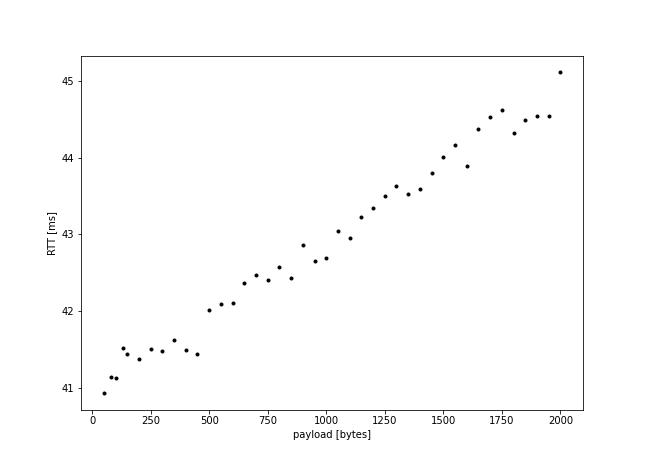
\includegraphics[width=\textwidth]{img/min.png}
         \caption{RTT minimo.}
         \label{fig:rttmin}
     \end{subfigure}
     \hfill
     \begin{subfigure}[b]{0.49\textwidth}
         \centering
         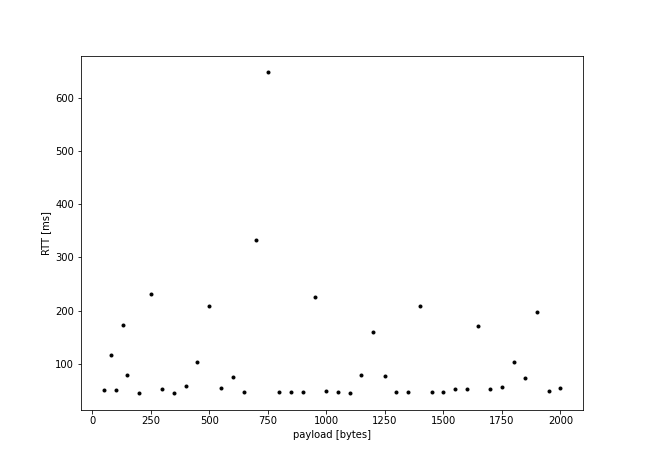
\includegraphics[width=\textwidth]{img/max.png}
         \caption{RTT massimo.}
         \label{fig:rttmax}
     \end{subfigure}
     \hfill
     \begin{subfigure}[b]{0.49\textwidth}
         \centering
         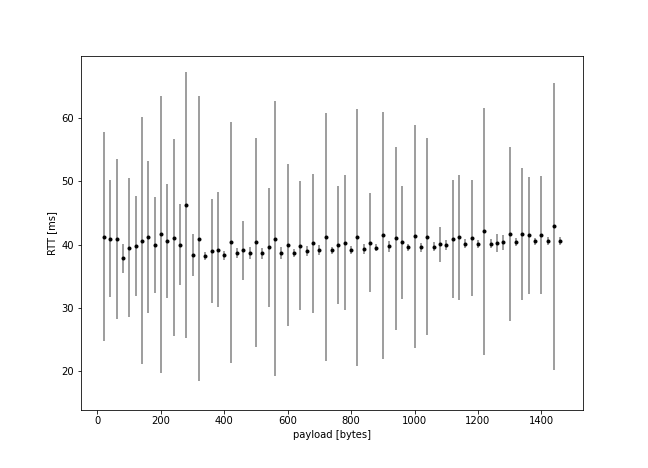
\includegraphics[width=\textwidth]{img/avg.png}
         \caption{RTT medio e relativa deviazione standard.}
         \label{fig:rttavg}
     \end{subfigure}
        \caption{Andamento del RTT al variare della dimensione del payload.}
        \label{fig:rttfig}
\end{figure}

\subsection{Bitrate}
Il bitrate della connessione può essere calcolato, grazie all'Equazione (\ref{eq:rtt1}), dai valori del RTT. Come è stato sperimentalmente verificato, i valori di RTT misurati con il comando \texttt{ping} normalmente variano, anche considerevolmente, per pacchetti diversi. Assumendo che il percorso tra sorgente e destinazione rimanga sempre lo stesso in prove consecutive (a parità di dimensione del pacchetto), la causa principale della variazione di RTT è da ricercarsi nel ritardo di accodamento. Per ridurre al minimo l'effetto di questa componente del ritardo consideriamo per ogni misurazione il RTT minimo, per cui questa componente è considerata nulla. Lavoriamo inoltre nell'ipotesi in cui il tempo di elaborazione dei vari nodi intermedi sia generalmente trascurabile. In queste condizioni, il bitrate della connessione può essere ricavato dal coefficiente angolare $\alpha$ dell'Equazione (\ref{eq:rtt}), che equivale a
\begin{align}
\alpha = 2 \cdot \sum_{i=1}^{n}  \frac{1}{R_i} \approx \frac{2}{min_i R_i}
\label{eq:ris}
\end{align}
Al fine di ricavare il coefficiente angolare è stata applicata la regressione lineare all'insieme di dati precedentemente raccolti sul RTT. Il risultato è riportato in Figura \ref{fig:regr} e può essere algebricamente espresso come
\begin{align}
RTT(k) = \alpha L(x) + \tau = 2.84 \cdot 10^{-7}  L(x) + 3.65 \cdot 10^{-2}
\end{align}
dove:
\begin{itemize}
\item $\alpha$ è il coefficiente angolare estrapolato
\item $\tau$ è l'intercetta estrapolata, che corrisponde alla somma dei tempi di propagazione di tutti i nodi (contati due volte, andata e ritorno)
\end{itemize}
\noindent
Il bitrate della connessione può quindi essere calcolato (sfruttando l'Equazione (\ref{eq:ris})) e risulta essere pari a 7 041 265 bps, ovvero \textbf{6.71 Mbps}. Al fine di verifica, si è provato ad eseguire la regressione lineare anche sui dati relativi al RTT medio. In questo caso, la retta estrapolata utilizzando l'intero set di dati si è dimostrata essere evidentemente incompatibile con quella ottenuta dai valori del RTT minimo. Tuttavia, eliminando dai valori considerati tutte le misurazioni con una deviazione standard troppo alta ($>10\,ms$) e le prime 20 misurazioni effettuate (di cui è già stato discusso il comportamento anomalo nella sezione \ref{par:x}), si è riusciti ad estrapolare una retta con una diversa intercetta (la cui differenza con del min potrebbe essere interpretata come \textit{ritardo di buffering medio}) ma stesso coefficiente angolare e, di conseguenza, stesso bitrate. Entrambe le rette estrapolate sono riportate in Figura \ref{fig:regr}.
\begin{figure}[h!]
     \centering
         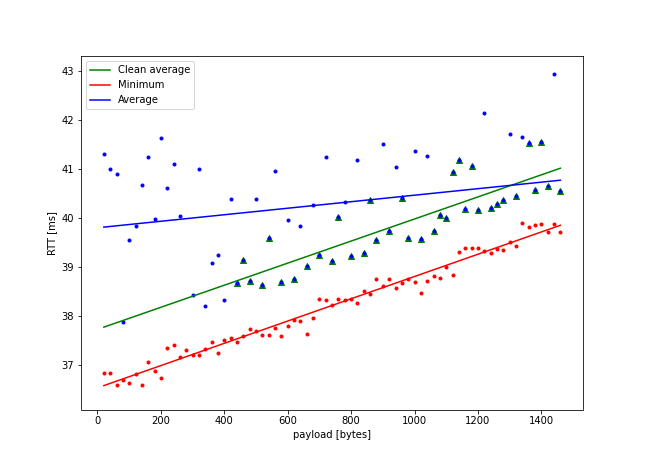
\includegraphics[scale=0.4]{img/clean.png}
         \vspace{-18pt}
         \caption{Regressioni lineari.}
         \label{fig:regr}
\end{figure}

\newpage

\section{Comando \texttt{iperf}}
\texttt{iperf} è un software client-server utilizzato nell'analisi delle prestazioni di rete per determinare il \textit{throughput} di un collegamento sfruttando TCP o UDP. L'applicativo deve essere inizialmente avviato nel server, dove rimane in attesa di richieste di connessione da parte del client, e successivamente nel client (in cui bisogna indicare l'indirizzo IP, il protocollo di livello di trasporto e il numero di porta da contattare). Il client invia quindi una certa quantità di dati (senza risposta da parte del server) e, al termine della sessione, client e server calcolano la velocità media di trasferimento e altre metriche utili nell'analisi delle prestazioni. 

\subsection{Opzione da linea di comando}
Il software \texttt{iperf} offre numerose opzioni da linea di comando. Una lista di queste ultime può essere ottenuta dall'utente mediante l'invocazione del comando \texttt{man ping}. Le opzioni che sono state utilizzate nello svolgimento dell'esperimento sono state:
\begin{itemize}
	\item \texttt{-s, --server}: run in server mode
	\item \texttt{-c, --client host}: run in client mode, connecting to host
	\item \texttt{-b, --bandwidth}: set the target bandwidth and optional standard devation per <mean>,[<stdev>]
	\item \texttt{-p, --port n}: set server port to listen on/connect to to n (default 5001)
	\item \texttt{-N, --nodelay}: set TCP no delay, disabling Nagle's Algorithm
	\item \texttt{-y, --reportstyle C|c}: if set to C or c report results as CSV (comma separated values)
\end{itemize}

\subsection{Bitrate}
Anche in questo caso, al fine di raccogliere un numero sufficiente di misure, è stato scritto uno script di shell Linux, riportato di seguito.
\small
\begin{quote}
\begin{verbatim}
echo "date,c_IP,c_port,s_ip,s_port,trans_ID,time,trans,bitrate" > iperf.csv
i=0
while [ $i -le 180 ]
do
  iperf -c 88.80.187.84 -p 20180 -b 100M -N -y c >> iperf.csv
  i=$(( $i + 1 ))
  sleep 2m
done
\end{verbatim}
\end{quote}
\normalsize
A differenza di \texttt{ping}, gli output di questo programma sono stati salvati (grazie all'opzione \texttt{-y c}) in formato csv, in modo tale da facilitarne una successiva elaborazione automatica. Il programma è stato avviato in modalità client (\texttt{-c}) sulla macchina da cui sono stati eseguiti i test ed in modalità server (tramite il comando \texttt{iperf -s -p 20180}) sul nodo di destinazione. Al lato client sono stati specificati indirizzo IP e porta del server destinazione (88.80.187.84 : 20180), mentre al lato server è stata specificato solamente il numero di porta su cui mettersi in ascolto.\\\\
È stata inoltre fissata lato client la "bandwidth" massima della connessione ad un limite molto superiore a quello effettivo (\texttt{-b 500M}, ossia 500 Mb), per evitare che il programma utilizzasse il valore di default corrispondente a 1.05 Mbps, falsando di conseguenza i risultati. Tramite il comando \texttt{sleep 2m} è stata inoltre definita una "pausa" tra le misurazioni successive del bitrate, in modo tale da aumentare il lasso di tempo di analisi e ridurre di conseguenza il peso di possibili congestioni temporanee della rete. Infine, è stata utilizzata l'opzione \texttt{-N} al fine di disattivare il buffering dei pacchetti di dimensione minore previsto dall'algoritmo di Nagle, che ha effetti sensibili sulla misura del bitrate.
\newpage

\noindent
Una rappresentazione grafica dei risultati ottenuti è riportata in Figura \ref{fig:iperf}. Il valore medio del bitrate misurato dal programma \texttt{iperf} risulta essere pari a \textbf{6.44 Mbps}.\\

\noindent
È stato tuttavia osservato nel corso degli esperimenti come questo valore sia in realtà altamente dipendente da alcuni parametri del programma, come ad esempio l'intervallo di tempo impostato per effettuare la misurazione. All'aumentare di questo parametro, infatti, si è osservata una decrescita esponenziale del bitrate, che converge per tempi lunghi ai valori di media trovati precedentemente (Figura \ref{fig:iperftime}). Questo risultato può essere spiegato se considerata l'equazione con la quale il programma calcola il bitrate, ossia
\begin{align}
\label{eq:br}
bitrate = \frac{bytes \ read}{time}
\end{align}
È possibile quindi che andando a ridurre il tempo di misurazione si riduca il denominatore ad un rate minore di quanto non si riduca il numeratore nello stesso intervallo. 
\begin{figure}[!htb]
   \begin{minipage}{0.48\textwidth}
     \centering
         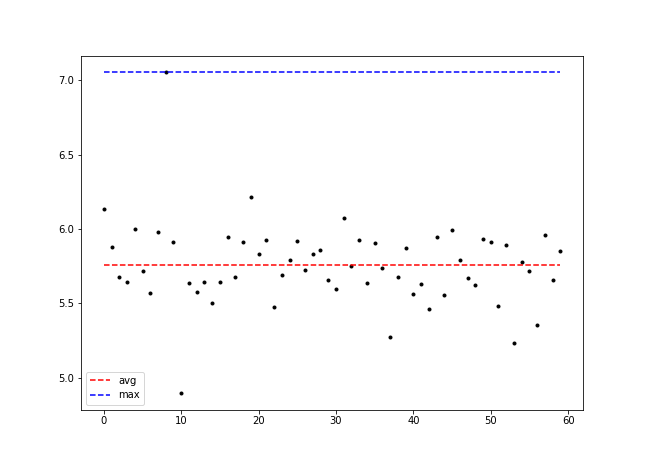
\includegraphics[width=1\linewidth]{img/iperf.png}
         \caption{Misure di bitrate della connessione.}
         \label{fig:iperf}
   \end{minipage}\hfill
   \begin{minipage}{0.48\textwidth}
      \centering
         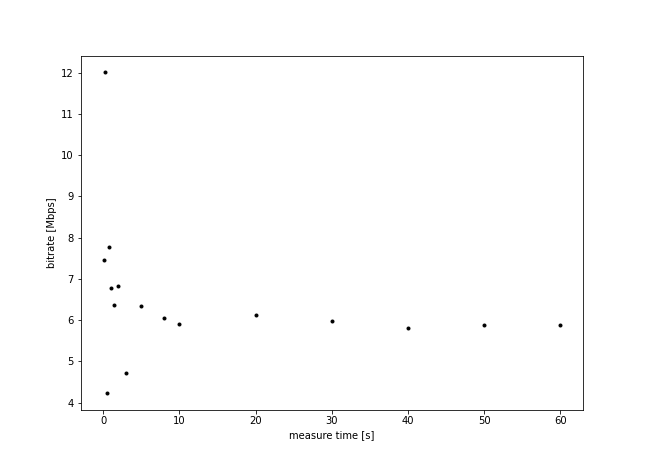
\includegraphics[width=1\linewidth]{img/iperftime.png}
         \caption{Bitrate in funzione del tempo.}
         \label{fig:iperftime}
   \end{minipage}
\end{figure}

\section{Conclusioni}
Le stime del bitrate ottenute mediante i due comandi \texttt{ping} e \texttt{iperf} sono tra loro molto simili e denotano una differenza reciproca inferiore al $5\%$, legata verosimilmente alle approssimazioni fatte nel calcolo della pendenza per i valori di bitrate del \texttt{ping} e agli errori casuali legati alla forte variabilità dello stato della rete. In conclusione, quindi, entrambi gli strumenti utilizzati hanno ottenuto risultati tra loro coerenti.

\section{Bibliografia}
\printbibliography[heading=none]

\end{document}